\documentclass[11pt,pdftex,portrait,letterpaper]{article}
\usepackage[hdivide={1in,*,1in},
            vdivide={1in,*,1in},
%            showframe
            ]{geometry}

\usepackage{graphicx}
\usepackage{longtable}
\usepackage{acronym}
\usepackage{verbatim}
\usepackage{subfigure}
\usepackage{fancyhdr}
\pagestyle{fancy}
\usepackage{listings}
\usepackage{color}
\usepackage{lastpage}

% Default margins are too wide all the way around. Reset them here
\setlength{\topmargin}{-.5in}
\setlength{\textheight}{9in}
\setlength{\oddsidemargin}{.125in}
\setlength{\textwidth}{6.25in}

\lhead{ECEN 498}
\chead{}
\rhead{\thepage\ of \pageref{LastPage}}
%\lfoot{\hline}
\lfoot{}
\cfoot{\small{University of Nebraska - Lincoln Department of Electrical Engineering}}
\rfoot{}
\renewcommand{\footrulewidth}{0.5pt}


% Modify parameters of Listings
\lstset{ 
language=C,
basicstyle=\scriptsize,
numbers=left,
numberstyle=\footnotesize,
stepnumber=1,
numbersep=10pt,
backgroundcolor=\color{white},
frame=single,
captionpos=b,
breaklines=true,
breakatwhitespace=false
}

\begin{document}

\vspace*{30ex}
\begin{center}

\textbf{Project 1 - NCO}\\

\vspace{4ex}
Real-Time Digital Signal Processing - University of Nebraska \\

\vspace{4ex}
Zach Swanson\\

\end{center}


\pagebreak
\tableofcontents
%\pagebreak
%\listoffigures
%\addcontentsline{toc}{section}{{\bf List of Figures}}
\pagebreak


\section{Introduction}

The purpose of this project was to gain introductory experience with the Texas Instruments (TI) ezDSP5535 (ezDSP) development board by designing and implementing a numerically controlled oscillator (NCO). This report will cover a brief background on NCO's, outline the project specifications, describe the program implemetation, and analyze the project results.

\section{Background}

An NCO is a digital signal generator capable of producing signals at various frequencies. NCOs operate using a M-bit phase accumulator and a lookup table (LUT). As the name describes, LUTs contain discrete values of a desired signal (e.g. a sinusoid) and the program can reference the LUT to look up a value in the table and return said value. The N most significant bits of the phase accumulator serve as the NCO's index for the LUT and the remaining \( M - N \) bits serve as "accumulation" bits. Because N-bits are used to index the LUT, the LUT is an array containing \(  2^N \) elements. The frequency of the signal generated by the NCO is controlled by how much the phase accumulator is increased, $\Delta$, each time through the NCO. The $\Delta$ value was calculated as \(\Delta =( {f}_{tone}*  2^N ) / {f}_{sample} \). Larger values of $\Delta$  allow the NCO to cycle through the LUT faster which corresponds to generating higher frequency signals. However, the NCO cannot generate a signal with a frequency higher than the sampling frequency. Another interesting characteristic of NCOs is that phase accumulator increases until it reaches its maximum value and then overflows. This allows the NCO to produce a periodic signal.

The NCO output is often passed to a  digital-to-analog converter (DAC) to create frequency-controlled analog output. 

\section{Project Description}

\subsection{Specifications}

The program for this project used portions of the \textbf{aic3204} program provided by TI that set up and initilialized the ezDSP's codec chip at a 48 kHz sample rate and tested the stereo in and out. The NCO was implemented using a M = 32 bit phase accumulator with N = 9 index bits. The NCO was implemented in a modular format, such that it could be used for later projects. 

Project deliverables included:
\begin{itemize}  
\item Oscilloscope captures of two signals at different frequencies
\item Accuracy of signal frequency
\item Range of frequency
\item Generate a chirp signal
\item Create signal attenuation function
\item Count cycles between adjacent writes to the DAC
\end{itemize}

\subsection{myNCO}

As specified, the key element of this project was creating a modular NCO function. The function implemented, myNCO, is shown in Listing \ref{l:myNCO}. The function took a desired frequency,  ${f}_{tone}$,  as a 16-bit unsigned integer input and returned a 16-bit signed integer value from a pre-generated lookup table. The frequency input was used to calculate the $\Delta$ value, \textit{paDelta}, to achieve the desired frequency as described in \textbf{Background}. The \textit{paDelta} value was added to the existing 32-bit unsigned integer phase accumulator variable, \textit{phaseAcc}. The \textit{phaseAcc} variable was declared as \textit{static} outside of myNCO to prevent redeclaring the variable each time the function was called and clearing the previous value. The index, \textit{lutIndex}, was obtained by right bit-shifting \textit{phaseAcc} 23 bits, i.e. the nine most significant bits were retained. The \textit{lookupTable} value at \textit{lutIndex} was returned from the function. 

\begin{lstlisting}[caption={Modular NCO function, myNCO}, label=l:myNCO]
static uint32_t phaseAcc = 0;

int16_t myNCO(uint16_t f_tone)
{
	uint32_t paDelta = (uint32_t) (f_tone * (0xFFFFFFFF / 48000));

	phaseAcc += paDelta;

	uint16_t lutIndex = (uint16_t)(phaseAcc >> 23);

	return lookupTable[lutIndex];
}
\end{lstlisting}

\subsection{Writing to the DAC}

Code from the \textbf{aic3204} program was used to set up the I2S peripheral for writing to the DAC and to write the code. Listing \ref{l:DAC} shows the portion of code borrowed to write the myNCO output to the DAC and subsequently the stereo out jack to generate a five-second tone. As mentioned previously, the codec was set at a sample rate of 48 kHz; hence, 48 samples would take approximately one millisecond. The nested for loop structure in Listing \ref{l:DAC} was based on 48 samples per millisecond. Therefore, myNCO was called every 1/48 millisecond and the return value was stored in a temporary variable, \textit{temp}, and written to the left 16-bit I2S channel and then the right channel. The code in Line 18 of Listing \ref{l:DAC} was how the chirp signal was generated. The chirp was accomplished by increasing the frequency of the NCO output every millisecond.

\begin{lstlisting}[caption={Snippet of code borrowed from aic3204 to write to DAC}, label=l:DAC]
    int16_t thisTone = 500;
  
    /* Play Tone for 5 seconds*/
    for ( sec = 0 ; sec < 5 ; sec++ )
    {
        for ( msec = 0 ; msec < 1000 ; msec++ )
        {
            for ( sample = 0 ; sample < 48 ; sample++ )
            {
                 int16_t temp = myNCO( thisTone );

                /* Write 16-bit left channel Data */
                EZDSP5535_I2S_writeLeft( temp );
                
                /* Write 16-bit right channel Data */
                EZDSP5535_I2S_writeRight( temp );
            }
            thisTone += 9;
        }
    }
\end{lstlisting}

\subsection{signalAttenuate}

To attenuate a given signal a function, signalAttenuate, was created. A signal, \textit{signal}, and a desired attenuation, \textit{attenuation}, were passed to the function and the signal was right bit-shifted  by the number of bits given by \textit{attenuation}. Extra care was taken because \textit{signal} was a signed integer, i.e. the most significant bit is a sign bit. Therefore, the if statement in Listing \ref{l:sigAtt} checked to see if \textit{signal} had a sign bit. If it had a sign bit, then the sign bit was set and the shifted sign bit was cleared after bit shifting \textit{signal}. If there was not a sign bit, then \textit{signal} was just bit shifted. The shifted \textit{signal} was returned from signalAttenuate as a signed 16-bit integer. 

\begin{lstlisting}[caption={Function to attenuate a given signal, signalAttenuate}, label=l:sigAtt]
int16_t signalAttenuate (int16_t signal, uint16_t attenuation)
{
	if ( signal & 0x8000000)
	{
		signal = signal >> attenuation;
		signal |= 0x80000000;
		signal &= 0x40000000;
	} else {
		signal = signal >> attenuation;
	}
	
	return signal;
}
\end{lstlisting}

\section{Results}

\subsection{Oscilloscope Captures}

Figures \ref{f:fig1} and \ref{f:fig2} show the oscilloscope captures of two generated signals at two kHz and ten kHz, respectively. As the Figures show, the NCO program was able to generate constant amplitude, constant frequency signals. 

\begin{figure}[h]
\centering
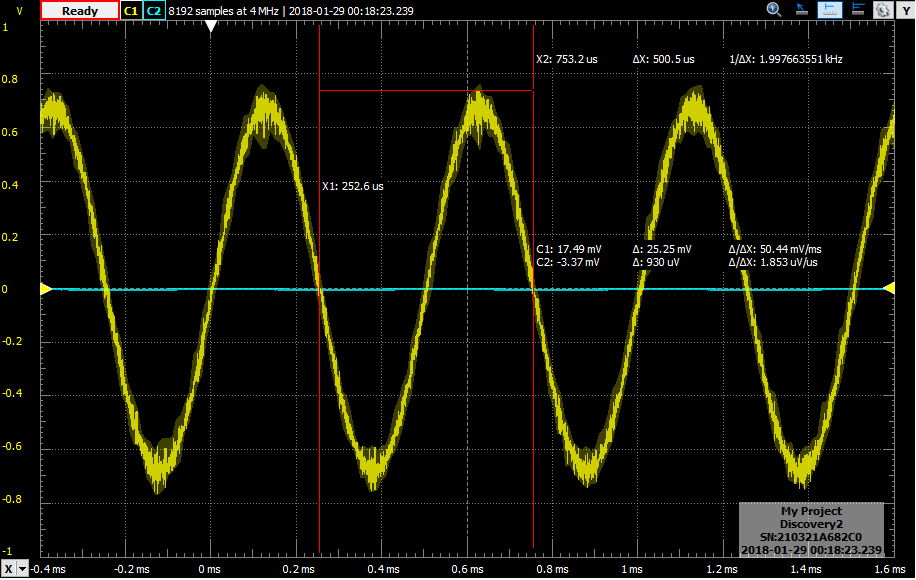
\includegraphics[width=0.8\textwidth]{./2000hzOscope}
\caption{Oscilloscope capture of 2 kHz sine wave}
\label{f:fig1}
\end{figure}

\begin{figure}[h]
\centering
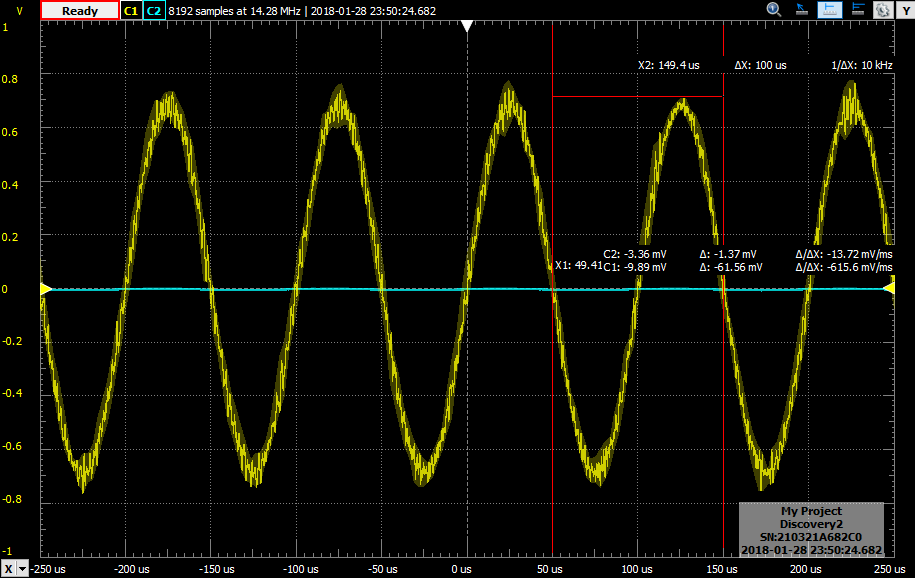
\includegraphics[width=0.8\textwidth]{./10000hzOscope}
\caption{Oscilloscope capture of 10 kHz sine wave}
\label{f:fig2}
\end{figure}

\subsection{Frequency Accuracy}

As seen in \textbf{Oscilloscope Captures}, the observed frequencies of the generated sine waves were very close to the expected frequencies. Ten measurements were taken at several frequencies ranging from one kHz to ten kHz and all generated frequencies had less than one percent error from the expected value. The maximum observed error in this range was 0.643 percent. However, as seen in Figures \ref{f:fig1} and \ref{f:fig2}, the generated signal appears to have less "smoothness." This was likely due to the fact that a complete period of the signal was being constructed with fewer data points at higher frequencies. The accuracy of the frequency generated depended on the N index bits used. If more index bits were used, then greater accuracy would be achieved. 

\subsection{Frequency Range}

Based on the sampling rate of 48 kHz, it was anticipated that the frequency generated could never exceed 48 kHz because $\Delta$ would be so large that it would not accurately index the LUT. However, even at 48 kHz, the index would jump over the entire table and only provide one data point from the LUT. To generate a recognizeable sine wave, it was hypothesized that at least three LUT values were needed. Therefore, the maximum frequency that would provide a good sine wave was estimated to be about 16,000 kHz. On the low frequency end, it seemed reasonable that a sine wave could be generated as low as 1 Hz (no lower because of integer format). However, the NCO would generate 512 index values at 176 Hz, so it was anticipated that at values below 176 Hz some distortion may appear. 

As expected signals with the correct frequency were generated down to 1 Hz; however, at frequencies below approximately 150 Hz the signals became uniformly attenuated. The maximum frequency that produced a good sine wave was approximately 21 kHz. Above this frequency the frequency error began to increase and the amplitude distortions appeared, as in Figure \ref{f:fig3}. 

\begin{figure}[h]
\centering
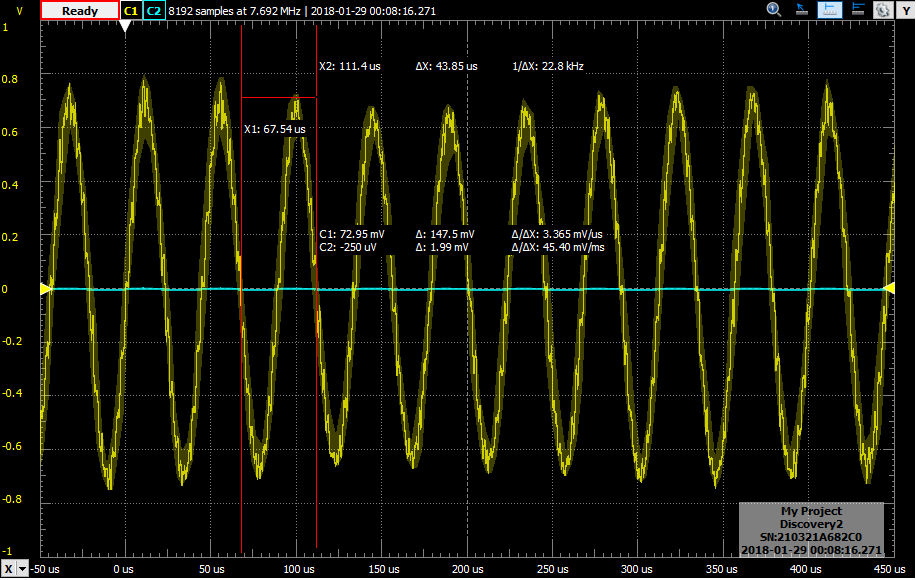
\includegraphics[width=0.8\textwidth]{./22500hzOscope}
\caption{Oscilloscope capture of 22.5 kHz sine wave}
\label{f:fig3}
\end{figure}

\subsection{Chirp}

Figure \ref{f:fig4} shows the "chirp" signal generated by the NCO program. The chirp sounded as expected, starting at a low frequency sound and growing to a high frequency sound. The shape of the chirp signal was interesting due to its decaying nature. It was also interesting that the decaying signal was periodic. It is unclear how exactly the shape was formed.

\begin{figure}[h]
\centering
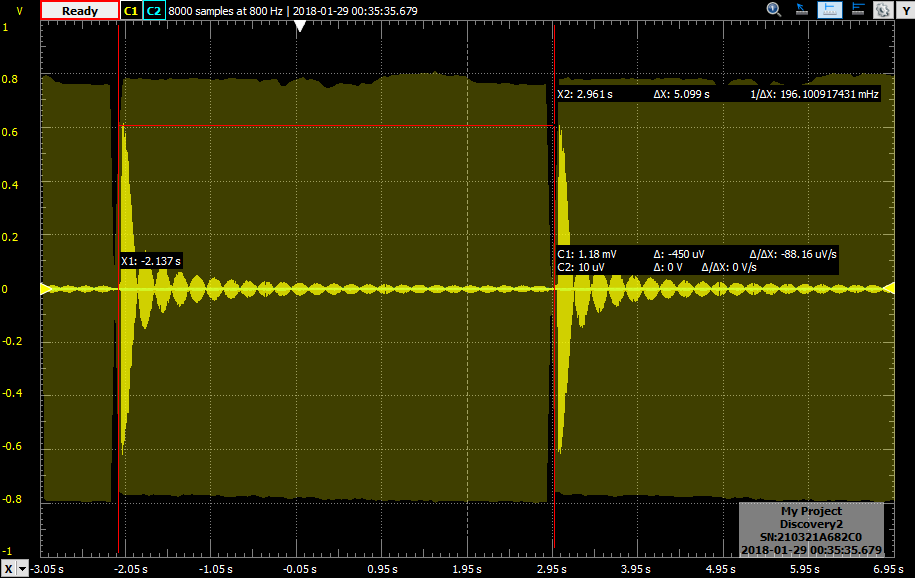
\includegraphics[width=0.8\textwidth]{./chirp}
\caption{Oscilloscope capture of "chirp" signal}
\label{f:fig4}
\end{figure}

\subsection{Attenuate}

Figure \ref{f:fig5} shows the attenuated signal generated using \textit{signalAttenuate( )}. As the Figure shows, several levels of attenuation were achieved by right bit-shifting the original signal values. Shifting by a bit corresponded to attenuation by a factor of two, which is expected because each bit is a power of two. 

\begin{figure}[h]
\centering
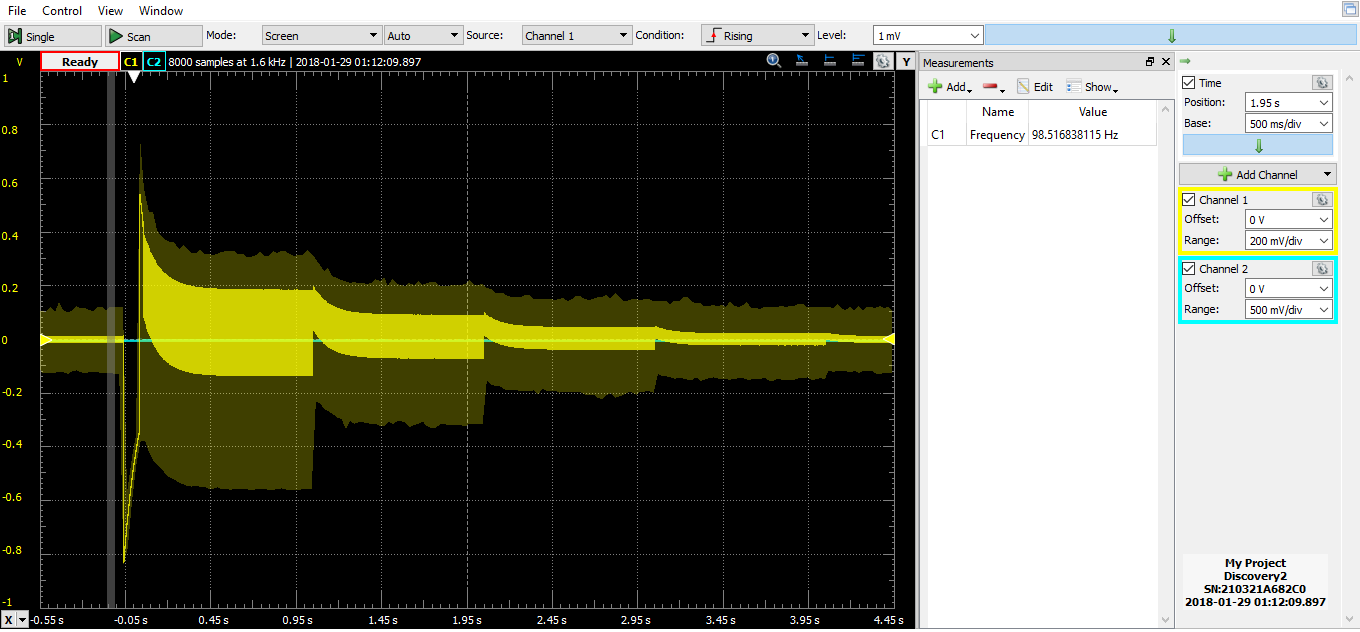
\includegraphics[width=0.8\textwidth]{./attenuate}
\caption{Oscilloscope capture of attenuated signal}
\label{f:fig5}
\end{figure}

\subsection{DAC Cycle Count}

The final deliverable for this project was not accomplished. Difficulty was encountered while attempting to use the Code Composer Studios (CCS) profile clock feature. The profile clock would not register clock cycles for any part of the program. Break points were set in various locations in an attempt to get the profile clock to observe cycles, but all attempts failed.

\pagebreak

\section{Appendix}

\begin{lstlisting}[caption={main}, label=l:main]
#include "stdio.h"
#include "ezdsp5535.h"
#include "ezdsp5535_gpio.h"
#include "ezdsp5535_i2c.h"

extern Int16 aic3204_tone_headphone( );

/*
 *
 *  main( )
 *
 */
void main( void )
{
    /* Initialize BSL */
    EZDSP5535_init( );


    /* Initialize I2C */
    EZDSP5535_I2C_init( );


    while(1)
    {
        /* Send tone to headphone */
        aic3204_tone_headphone( );

        EZDSP5535_wait( 100 );  // Wait
    }
}
\end{lstlisting}

\pagebreak

\begin{lstlisting}[caption={aic3204 tone headphone}, label=l:aic3204]
#include "stdio.h"
#include "stdint.h"
#include "ezdsp5535.h"
#include "ezdsp5535_i2s.h"
#include "csl_i2s.h"
#include "myNCO.h"

extern Int16 AIC3204_rset( Uint16 regnum, Uint16 regval);

/*
 *  AIC3204 Tone 
 *      Output a 1 kHz tone through the LINE OUT
 */
Int16 aic3204_tone_headphone( )
{
    Int16 sec, msec;
    Int16 sample;

    /* Configure AIC3204 */
    AIC3204_rset( 0,  0x00 );  // Select page 0
    AIC3204_rset( 1,  0x01 );  // Reset codec
    EZDSP5535_waitusec(1000);  // Wait 1ms after reset
    AIC3204_rset( 0,  0x01 );  // Select page 1
    AIC3204_rset( 1,  0x08 );  // Disable crude AVDD generation from DVDD
    AIC3204_rset( 2,  0x01 );  // Enable Analog Blocks, use LDO power
    AIC3204_rset( 123,0x05 );  // Force reference to power up in 40ms
    EZDSP5535_waitusec(50000); // Wait at least 40ms
    AIC3204_rset( 0,  0x00 );  // Select page 0
    
    /* PLL and Clocks config and Power Up  */
    AIC3204_rset( 27, 0x0d );  // BCLK and WCLK are set as o/p; AIC3204(Master)
    AIC3204_rset( 28, 0x00 );  // Data ofset = 0
    AIC3204_rset( 4,  0x03 );  // PLL setting: PLLCLK <- MCLK, CODEC_CLKIN <-PLL CLK
    AIC3204_rset( 6,  0x07 );  // PLL setting: J=7
    AIC3204_rset( 7,  0x06 );  // PLL setting: HI_BYTE(D=1680)
    AIC3204_rset( 8,  0x90 );  // PLL setting: LO_BYTE(D=1680)
    AIC3204_rset( 30, 0x88 );  // For 32 bit clocks per frame in Master mode ONLY
                               // BCLK=DAC_CLK/N =(12288000/8) = 1.536MHz = 32*fs
    AIC3204_rset( 5,  0x91 );  // PLL setting: Power up PLL, P=1 and R=1
    EZDSP5535_waitusec(10000); // Wait for PLL to come up    
    AIC3204_rset( 13, 0x00 );  // Hi_Byte(DOSR) for DOSR = 128 decimal or 0x0080 DAC oversamppling
    AIC3204_rset( 14, 0x80 );  // Lo_Byte(DOSR) for DOSR = 128 decimal or 0x0080
    AIC3204_rset( 20, 0x80 );  // AOSR for AOSR = 128 decimal or 0x0080 for decimation filters 1 to 6
    AIC3204_rset( 11, 0x82 );  // Power up NDAC and set NDAC value to 2
    AIC3204_rset( 12, 0x87 );  // Power up MDAC and set MDAC value to 7
    AIC3204_rset( 18, 0x87 );  // Power up NADC and set NADC value to 7
    AIC3204_rset( 19, 0x82 );  // Power up MADC and set MADC value to 2
    
    /* DAC ROUTING and Power Up */
    AIC3204_rset( 0,  0x01 );  // Select page 1
    AIC3204_rset( 12, 0x08 );  // LDAC AFIR routed to HPL
    AIC3204_rset( 13, 0x08 );  // RDAC AFIR routed to HPR
    AIC3204_rset( 0,  0x00 );  // Select page 0
    AIC3204_rset( 64, 0x02 );  // Left vol=right vol
    AIC3204_rset( 65, 0x00 );  // Left DAC gain to 0dB VOL; Right tracks Left
    AIC3204_rset( 63, 0xd4 );  // Power up left,right data paths and set channel
    AIC3204_rset( 0,  0x01 );  // Select page 1
    AIC3204_rset( 16, 0x00 );  // Unmute HPL , 0dB gain
    AIC3204_rset( 17, 0x00 );  // Unmute HPR , 0dB gain
    AIC3204_rset( 9 , 0x30 );  // Power up HPL,HPR
    EZDSP5535_waitusec(100 );  // Wait
    
    /* ADC ROUTING and Power Up */
    AIC3204_rset( 0,  0x01 );  // Select page 1
    AIC3204_rset( 52, 0x30 );  // STEREO 1 Jack
                               // IN2_L to LADC_P through 40 kohm
    AIC3204_rset( 55, 0x30 );  // IN2_R to RADC_P through 40 kohmm
    AIC3204_rset( 54, 0x03 );  // CM_1 (common mode) to LADC_M through 40 kohm
    AIC3204_rset( 57, 0xc0 );  // CM_1 (common mode) to RADC_M through 40 kohm
    AIC3204_rset( 59, 0x00 );  // MIC_PGA_L unmute
    AIC3204_rset( 60, 0x00 );  // MIC_PGA_R unmute
    AIC3204_rset( 0,  0x00 );  // Select page 0
    AIC3204_rset( 81, 0xc0 );  // Powerup Left and Right ADC
    AIC3204_rset( 82, 0x00 );  // Unmute Left and Right ADC
    AIC3204_rset( 0,  0x00 );  // Select page 0 
    EZDSP5535_waitusec(100 );  // Wait

    /* Initialize I2S */
    EZDSP5535_I2S_init();

    uint16_t thisTone = 1000;
    uint16_t thisAttenuation = 0;
  
    /* Play Tone for 5 seconds*/
    for ( sec = 0 ; sec < 5 ; sec++ )
    {
        for ( msec = 0 ; msec < 1000 ; msec++ )
        {
            for ( sample = 0 ; sample < 48 ; sample++ )
            {
            	int16_t temp = myNCO( thisTone );
            	//temp = signalAttenuate(temp, thisAttenuation);

                /* Write 16-bit left channel Data */
                EZDSP5535_I2S_writeLeft( temp );
                
                /* Write 16-bit right channel Data */
                EZDSP5535_I2S_writeRight( temp );
            }
            //thisTone += 4;
        }

        //thisAttenuation++;
    }
    EZDSP5535_I2S_close();    // Disble I2S
    AIC3204_rset( 0,  0x00 );  // Select page 0
    AIC3204_rset( 1,  0x01 );  // Reset codec
    
    return 0;
}
\end{lstlisting}

\pagebreak

\begin{lstlisting}[caption={myNCO}, label=l:myNCO]
#include "stdint.h"

/* Pre-generated sine wave data, 16-bit signed samples */
static int16_t lookupTable[] = {
         0,    402,    804,   1206,   1608,   2009,   2411,   2811,   3212,   3612,   4011,   4410,   4808,   5205,   5602,   5998,
      6393,   6787,   7180,   7571,   7962,   8351,   8740,   9127,   9512,   9896,  10279,  10660,  11039,  11417,  11793,  12167,
     12540,  12910,  13279,  13646,  14010,  14373,  14733,  15091,  15447,  15800,  16151,  16500,  16846,  17190,  17531,  17869,
     18205,  18538,  18868,  19195,  19520,  19841,  20160,  20475,  20788,  21097,  21403,  21706,  22006,  22302,  22595,  22884,
     23170,  23453,  23732,  24008,  24279,  24548,  24812,  25073,  25330,  25583,  25833,  26078,  26320,  26557,  26791,  27020,
     27246,  27467,  27684,  27897,  28106,  28311,  28511,  28707,  28899,  29086,  29269,  29448,  29622,  29792,  29957,  30118,
     30274,  30425,  30572,  30715,  30853,  30986,  31114,  31238,  31357,  31471,  31581,  31686,  31786,  31881,  31972,  32058,
     32138,  32214,  32286,  32352,  32413,  32470,  32522,  32568,  32610,  32647,  32679,  32706,  32729,  32746,  32758,  32766,
     32767,  32766,  32758,  32746,  32729,  32706,  32679,  32647,  32610,  32568,  32522,  32470,  32413,  32352,  32286,  32214,
     32138,  32058,  31972,  31881,  31786,  31686,  31581,  31471,  31357,  31238,  31114,  30986,  30853,  30715,  30572,  30425,
     30274,  30118,  29957,  29792,  29622,  29448,  29269,  29086,  28899,  28707,  28511,  28311,  28106,  27897,  27684,  27467,
     27246,  27020,  26791,  26557,  26320,  26078,  25833,  25583,  25330,  25073,  24812,  24548,  24279,  24008,  23732,  23453,
     23170,  22884,  22595,  22302,  22006,  21706,  21403,  21097,  20788,  20475,  20160,  19841,  19520,  19195,  18868,  18538,
     18205,  17869,  17531,  17190,  16846,  16500,  16151,  15800,  15447,  15091,  14733,  14373,  14010,  13646,  13279,  12910,
     12540,  12167,  11793,  11417,  11039,  10660,  10279,   9896,   9512,   9127,   8740,   8351,   7962,   7571,   7180,   6787,
      6393,   5998,   5602,   5205,   4808,   4410,   4011,   3612,   3212,   2811,   2411,   2009,   1608,   1206,    804,    402,
         0,   -402,   -804,  -1206,  -1608,  -2009,  -2411,  -2811,  -3212,  -3612,  -4011,  -4410,  -4808,  -5205,  -5602,  -5998,
     -6393,  -6787,  -7180,  -7571,  -7962,  -8351,  -8740,  -9127,  -9512,  -9896, -10279, -10660, -11039, -11417, -11793, -12167,
    -12540, -12910, -13279, -13646, -14010, -14373, -14733, -15091, -15447, -15800, -16151, -16500, -16846, -17190, -17531, -17869,
    -18205, -18538, -18868, -19195, -19520, -19841, -20160, -20475, -20788, -21097, -21403, -21706, -22006, -22302, -22595, -22884,
    -23170, -23453, -23732, -24008, -24279, -24548, -24812, -25073, -25330, -25583, -25833, -26078, -26320, -26557, -26791, -27020,
    -27246, -27467, -27684, -27897, -28106, -28311, -28511, -28707, -28899, -29086, -29269, -29448, -29622, -29792, -29957, -30118,
    -30274, -30425, -30572, -30715, -30853, -30986, -31114, -31238, -31357, -31471, -31581, -31686, -31786, -31881, -31972, -32058,
    -32138, -32214, -32286, -32352, -32413, -32470, -32522, -32568, -32610, -32647, -32679, -32706, -32729, -32746, -32758, -32766,
    -32768, -32766, -32758, -32746, -32729, -32706, -32679, -32647, -32610, -32568, -32522, -32470, -32413, -32352, -32286, -32214,
    -32138, -32058, -31972, -31881, -31786, -31686, -31581, -31471, -31357, -31238, -31114, -30986, -30853, -30715, -30572, -30425,
    -30274, -30118, -29957, -29792, -29622, -29448, -29269, -29086, -28899, -28707, -28511, -28311, -28106, -27897, -27684, -27467,
    -27246, -27020, -26791, -26557, -26320, -26078, -25833, -25583, -25330, -25073, -24812, -24548, -24279, -24008, -23732, -23453,
    -23170, -22884, -22595, -22302, -22006, -21706, -21403, -21097, -20788, -20475, -20160, -19841, -19520, -19195, -18868, -18538,
    -18205, -17869, -17531, -17190, -16846, -16500, -16151, -15800, -15447, -15091, -14733, -14373, -14010, -13646, -13279, -12910,
    -12540, -12167, -11793, -11417, -11039, -10660, -10279,  -9896,  -9512,  -9127,  -8740,  -8351,  -7962,  -7571,  -7180,  -6787,
     -6393,  -5998,  -5602,  -5205,  -4808,  -4410,  -4011,  -3612,  -3212,  -2811,  -2411,  -2009,  -1608,  -1206,   -804,   -402
};

static uint32_t phaseAcc = 0;

int16_t myNCO(uint16_t f_tone)
{
	uint32_t paDelta = (uint32_t) (f_tone * (0xFFFFFFFF / 48000));

	phaseAcc += paDelta;

	uint16_t lutIndex = (uint16_t)(phaseAcc >> 23);

	return lookupTable[lutIndex];
}



int16_t signalAttenuate (int16_t signal, uint16_t attenuation)
{
	if ( signal & 0x8000000)
	{
		signal = signal >> attenuation;
		signal |= 0x80000000;
		signal &= 0x40000000;
	} else {
		signal = signal >> attenuation;
	}

	return signal;
}
\end{lstlisting}

\end{document}



